\documentclass[12pt]{article}
\usepackage{graphicx}
\usepackage[left=3cm,top=3cm,right=3cm,bottom=3cm]{geometry}

\begin{document}

\title{Bayesian Inference of Species Trees from Multilocus Data using *BEAST }

\author{Alexei J Drummond, Walter Xie and Joseph Heled}

\date{\today{}}

\maketitle

\section*{Introduction}

We describe a full Bayesian framework for species tree estimation. We have attempted to combine the best aspects of previous methods to provide joint inference of a species tree topology, divergence times, population sizes, and gene trees from multiple genes sampled from multiple individuals across a set of closely related species. We have achieved this by extending BEAST to *BEAST (pronounced "star beast"), which is published below:

Joseph Heled and Alexei J. Drummond
Bayesian Inference of Species Trees from Multilocus Data
Mol. Biol. Evol. 2010 27: 570-580. 

You will need the following software at your disposal:

\begin{itemize}

\item {\bf BEAST} - this package contains the BEAST program, BEAUti, TreeAnnotator and other utility programs. This tutorial is written for BEAST v1.7.x, which is available for download from  \texttt{http://beast.bio.ed.ac.uk/}.
\item {\bf Tracer} - this program is used to explore the output of BEAST (and other Bayesian MCMC programs). It graphically and
quantitively summarizes the distributions of continuous parameters and provides diagnostic information. At the time of
writing, the current version is v1.5. It is available for download from \texttt{http://beast.bio.ed.ac.uk/}.
\item {\bf FigTree} - this is an application for displaying and printing molecular phylogenies, in particular those obtained using
BEAST. At the time of writing, the current version is v1.3.1. It is available for download from \texttt{http://tree.bio.ed.ac.uk/}.
\end{itemize}

%%%%%%%%%%%%%%%%%%%%%%%%%%%%%%%%%%%%%%%%%%%%%
%%%
%%% TUTORIAL - *BEAST
%%%
%%%%%%%%%%%%%%%%%%%%%%%%%%%%%%%%%%%%%%%%%%%%%

\section*{*BEAST}

This tutorial will guide you through the analysis of three loci sampled from 26 individuals representing nine species of pocket gophers. This is a subset of previous published data \cite{belfiore2008multilocus}. The objective of this tutorial is to estimate the species tree that is most probable given the multi-individual multi-locus sequence data. The species tree has 9 taxa, whereas each gene tree has 26 taxa. *BEAST will co-estimate three gene trees embedded in a shared species tree (see Heled and Drummond, 2010 for details).

The first step will be to convert a NEXUS file with a DATA or CHARACTERS block into a BEAST XML input file. This is done using the program BEAUti (Bayesian Evolutionary Analysis Utility). This is a user-friendly program for setting the evolutionary model and options for the MCMC analysis. The second step is to actually run BEAST using the input file that contains the data, model and settings. The final step is to explore the output of BEAST in order to diagnose problems and to summarize the results.

\subsection*{BEAUti}

Run BEAUti by double clicking on its icon. 

\subsubsection*{Loading the NEXUS file }

To load a NEXUS format alignment, simply select the \texttt{Import
Data...} option from the File menu: 

\medskip{}

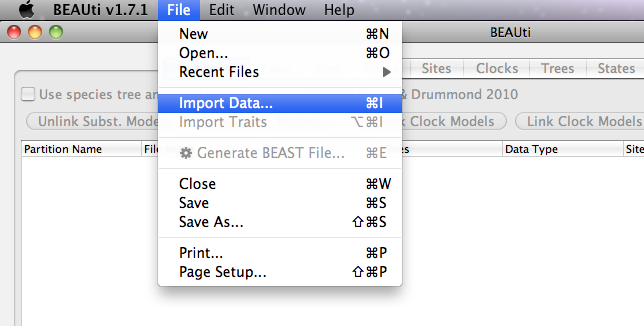
\includegraphics[scale=0.5]{figures/ImportNexus}

\medskip{}

Select three files called \texttt{26.nex, 29.nex, 47.nex} by holding \texttt{shift} key. Each file contains an alignment of sequences of from an independent locus. The \texttt{26.nex} looks like this (content has been truncated):

\begin{verbatim}
#NEXUS
[TBO26oLong]
BEGIN DATA;
	DIMENSIONS  NTAX =26 NCHAR=614;
	FORMAT DATATYPE = DNA GAP = - MISSING = ?;
	MATRIX	
	Orthogeomys_heterodus        ATTCTAGGCAAAAAGAGCAATGC ...
	Thomomys_bottae_awahnee_a    ????????????????????ATGCTG ...
	Thomomys_bottae_awahnee_b    ????????????????????ATGCTG ...
	Thomomys_bottae_xerophilus   ????????????????????ATGCTG ...
	Thomomys_bottae_cactophilus  ????????????????AGCAATGCT ...

         ... ...

;
END;
\end{verbatim}

\medskip{}

Once loaded, the three partitions are displayed in the main panel:

\medskip{}

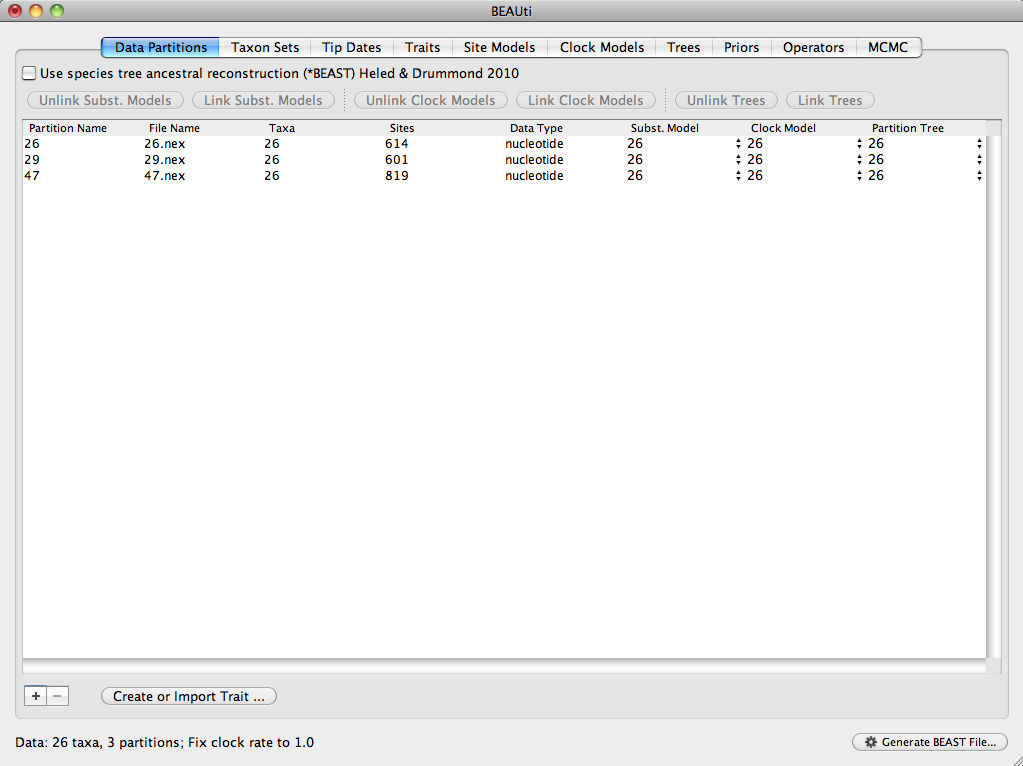
\includegraphics[scale=0.4]{figures/BEAUti_DataPartitions}

\medskip{}

Double click any alignment (partition) to show its detail:

\medskip{}

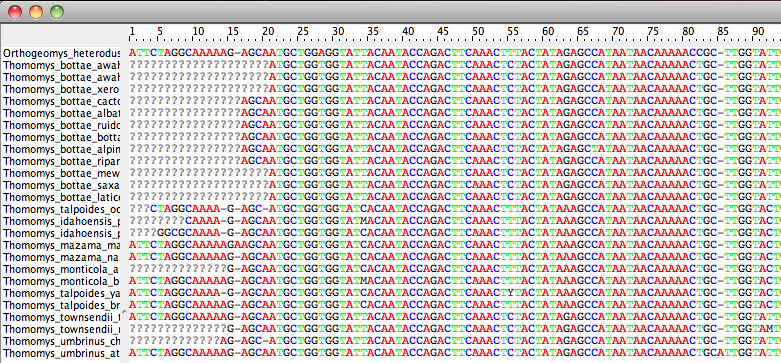
\includegraphics[scale=0.4]{figures/BEAUti_ShowAlignment}

\medskip{}

\subsubsection*{Import trait(s) from a mapping file to fire *BEAST}

To enable *BEAST in BEAST v1.7.x, simply click the check box labelled \texttt{Use species tree ancestral reconstruction (*BEAST) Heled \& Drummond 2010} on the top of {\bf Data Partitions} panel. Then, a {\bf Create or Import Trait(s)} dialog will pop up.   

\medskip{}

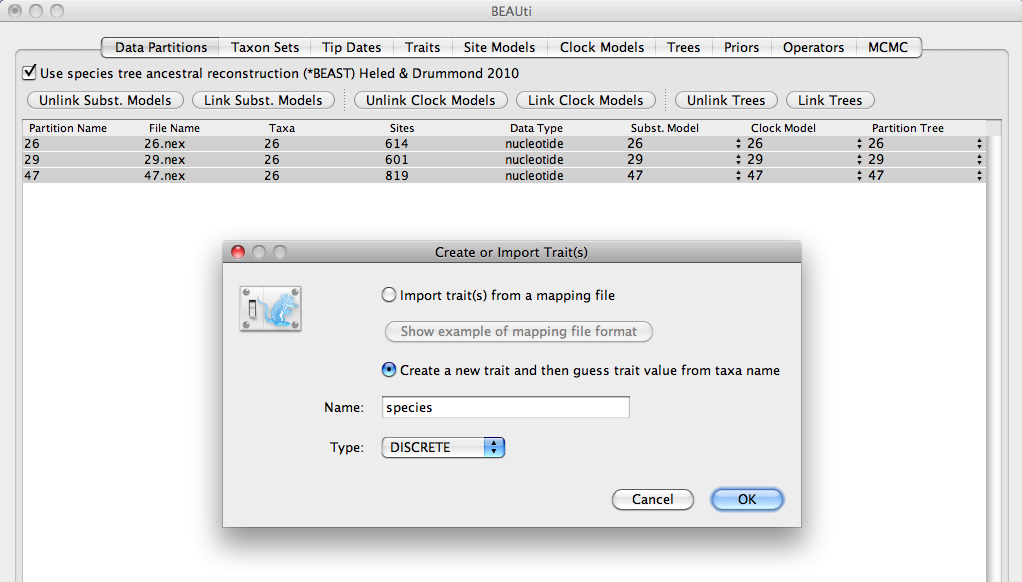
\includegraphics[scale=0.4]{figures/BEAUti_CreateImportTrait}

\medskip{}

There are two options to be selected: 
\begin{enumerate}
  \item Import trait(s) from a mapping file; 
  \item Create a new trait and then guess trait value from taxa name \texttt{species}.  
\end{enumerate}

Choose the first option and click \textbf{OK} to load the mapping file, named\\ \texttt{gopher\_mapping.txt}. 

Once loaded, a message indicating the use of *BEAST will be displayed in the status at the bottom of the window, and a trait named \texttt{species} is created in the trait table in the {\bf Traits} tab. Click it to show trait values. 

\medskip{}

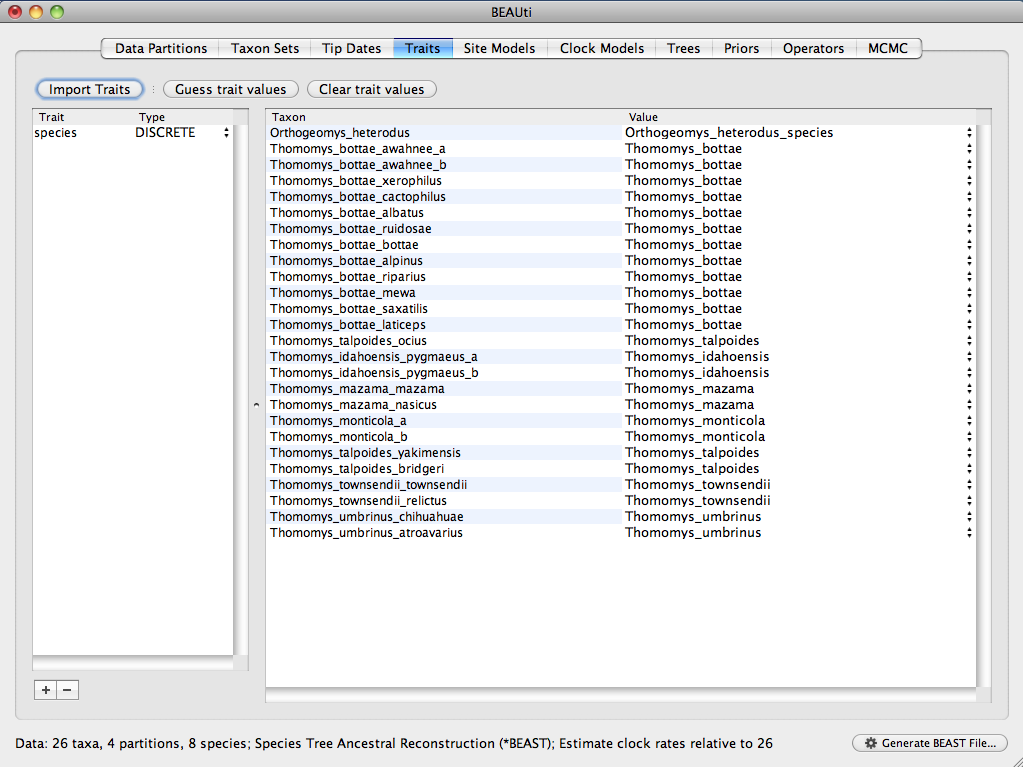
\includegraphics[scale=0.4]{figures/BEAUti_Trait}

\medskip{}

A proper trait file is tab delimited. The first row is always \texttt{traits} followed by the keyword \texttt{species} in the second column and separated by tab. The rest of the rows map each individual taxon name to a species name: the taxon name in the first column and species name in the second column separated by tab. For example:

\begin{verbatim}
traits	species
taxon1	speciesA
taxon2	speciesA
taxon3	speciesB
... ...
\end{verbatim}

For multi-locus analyses, BEAST can link or unlink substitutions models across the loci by clicking buttons on the top of {\bf Data Partitions} panel. The default of *BEAST is unlinking all models: substitution model, clock model, and tree models. Note that you should only unlink the tree model across data partitions that are actually genetically unlinked. For example, in most organisms all the mitochondrial genes are effectively linked due to a lack of recombination and they should be set up to use the same tree model in a *BEAST analysis. 

\medskip{}

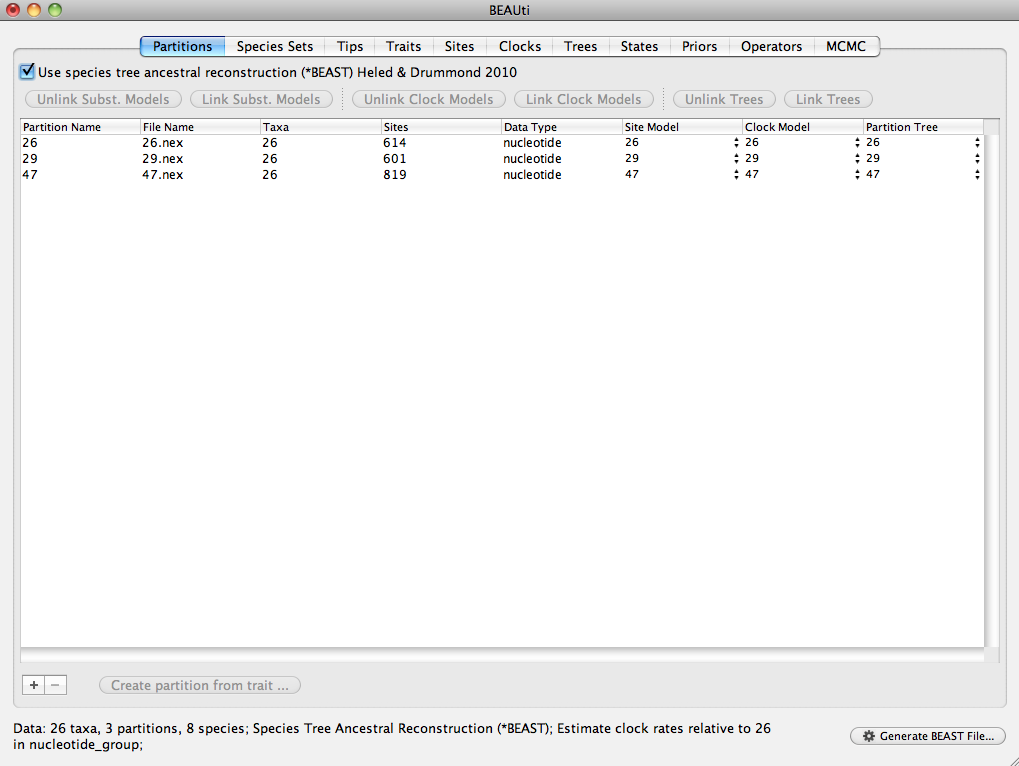
\includegraphics[scale=0.4]{figures/BEAUti_DataPartitions2}

\medskip{}


\subsubsection*{Alternatively: Create a species trait from taxa names}

The advantage of using the {\bf Traits} panel is that we can extract species names from the taxa names if they already contain that information. Let's go to {\bf Data Partitions} panel and unselect the check box labelled \texttt{Use species tree ancestral reconstruction (*BEAST) Heled \& Drummond 2010}. As we can see in the status bar on the bottom, the analysis has been reverted to a standard BEAST analysis.

To enable *BEAST again, click the \texttt{Use species tree ancestral reconstruction (*BEAST) Heled \& Drummond 2010} on the top of {\bf Data Partitions} panel, and then choose the second option in {\bf Create or Import Trait(s)} dialog this time. Click \textbf{OK} to continue, and then we will get to {\bf Traits} panel and click on the \textbf{Guess trait values} at the top to pop out {\bf Guess Trait Value for Taxa} dialog. Choose \textbf{second} in the drop list of \textbf{Defined by its order}, and input \textbf{\_} as separator. Click \textbf{OK}, and *BEAST is applied again.

\medskip{}

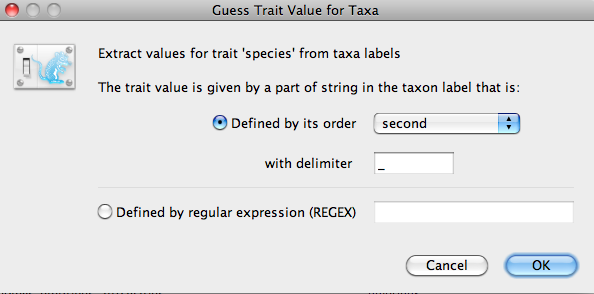
\includegraphics[scale=0.4]{figures/BEAUti_GuessTrait}

\medskip{}

\medskip{}

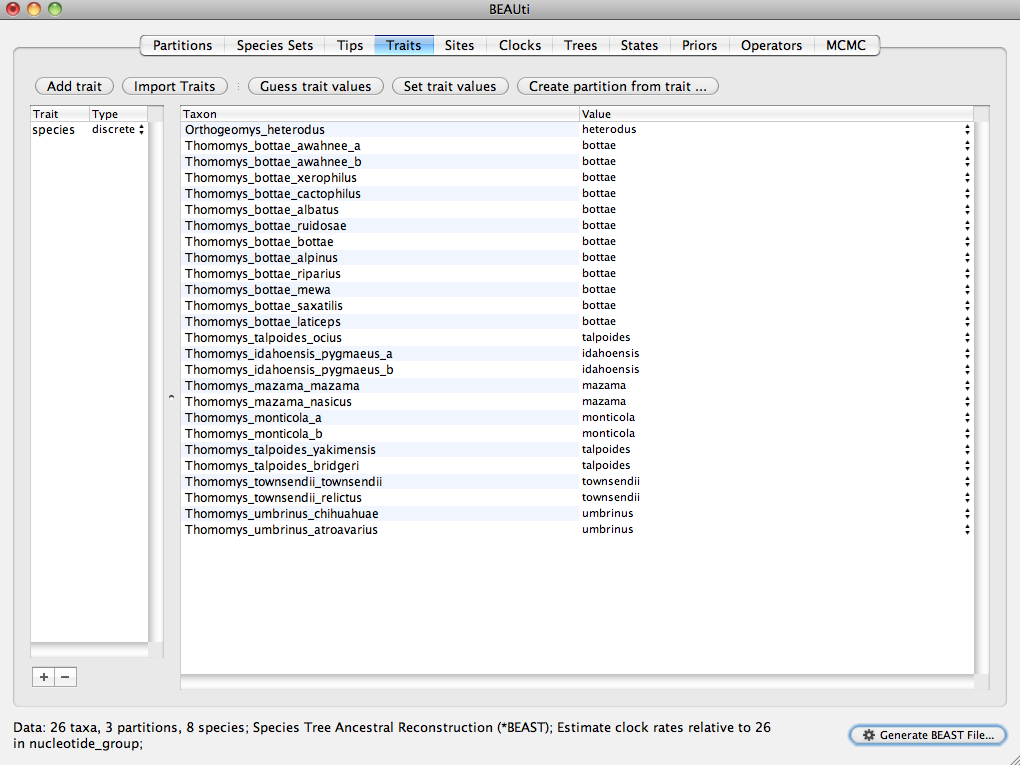
\includegraphics[scale=0.4]{figures/BEAUti_Trait2}

\medskip{}

\subsubsection*{Setting the substitution model}

The next thing to do is to click on the {\bf Site Models} tab at the top of the
main window. This will reveal the evolutionary model settings for
BEAST. Exactly which options appear depend on whether the data are
nucleotides, or amino acids, or binary data, or general data.
The settings that will appear after loading the data set will
be the default values so we need to make some changes. 

Most of the models should be familiar to you. For this analysis, we
will select each substitution model listed on the 
left side in turn to make the following change: select \textbf{Empirical} for the 
\textbf{Base frequencies}. {\it Remember to do this for all site models.}
\medskip{}

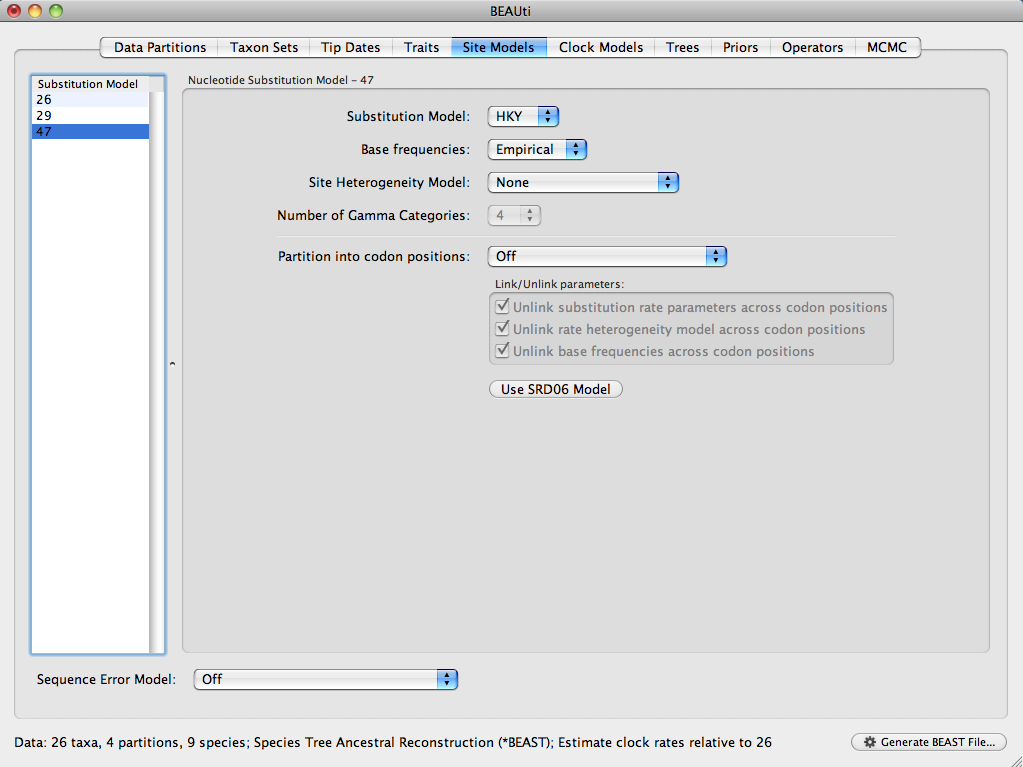
\includegraphics[scale=0.4]{figures/BEAUti_SiteModel}

\medskip{}

\subsubsection*{Setting the clock model}

Second, click on the {\bf Clock Models} tab at the top of the
main window. In this analysis, we use the \textbf{Strict Clock} molecular clock model as default.
Your model options should now look like this: 

\medskip{}

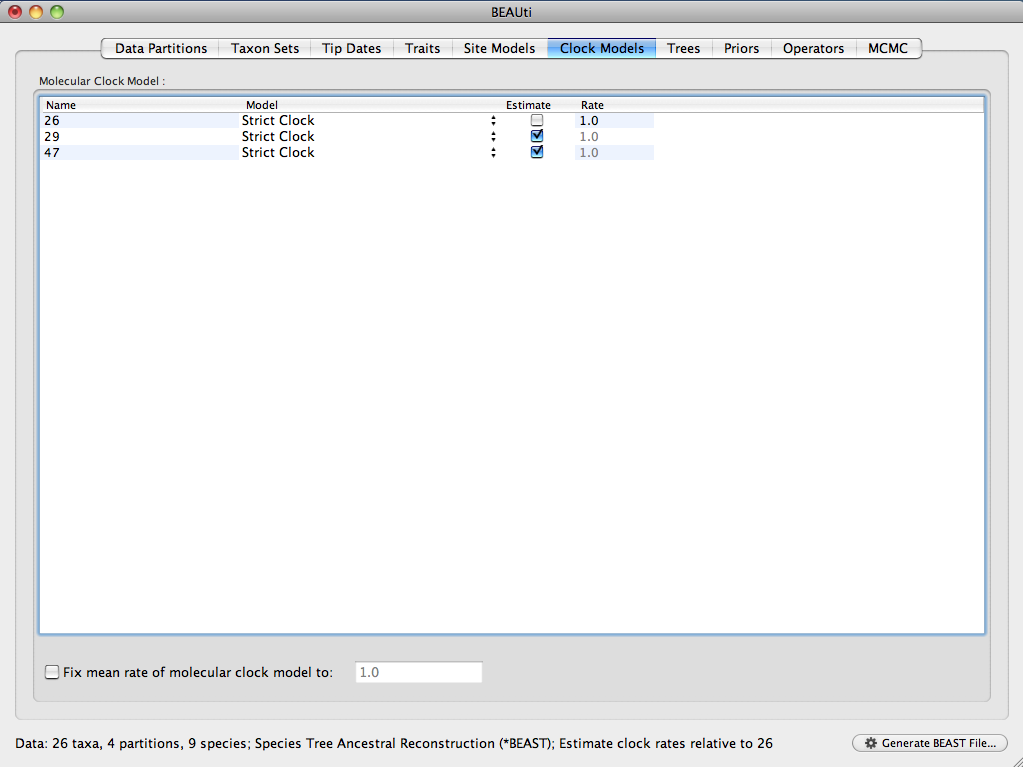
\includegraphics[scale=0.4]{figures/BEAUti_Clock}

\medskip{}

The \textbf{Estimate} check box is unchecked for the first clock model and checked for the rest clock models, because we wish to estimate the mutation rate of each subsequent locus relative to the first locus whose rate is fixed to 1.0. 

\subsubsection*{Trees}

The {\bf Trees} panel allows priors to be specified for each parameter in the model, which can be defined on the top of the panel. *BEAST has a different tree prior panel where users can only configure the species tree prior not gene tree priors (which are automatically specified by the multispecies coalescent). Currently, we have two species tree priors: \textbf{Yule Process} and \textbf{Birth-Death Process}; and three population size models: \textbf{Piecewise linear and constant root}, \textbf{Piecewise linear}, and \textbf{Piecewise constant}. In this analysis, we use the default options.

The bottom right panel is used to configure the corresponding starting trees. The \textbf{Ploidy Type} menu determines the type of sequence (mitochondrial, nuclear, X, Y). This matters since different modes of inheritance give rise to different effective population sizes. The \textbf{Starting Tree} menu provides three options, where the \textbf{user-specified} starting tree has to be loaded from the data file (e.g. NEXUS file) in advance. In this analysis, we simply use a random starting tree. 

\medskip{}

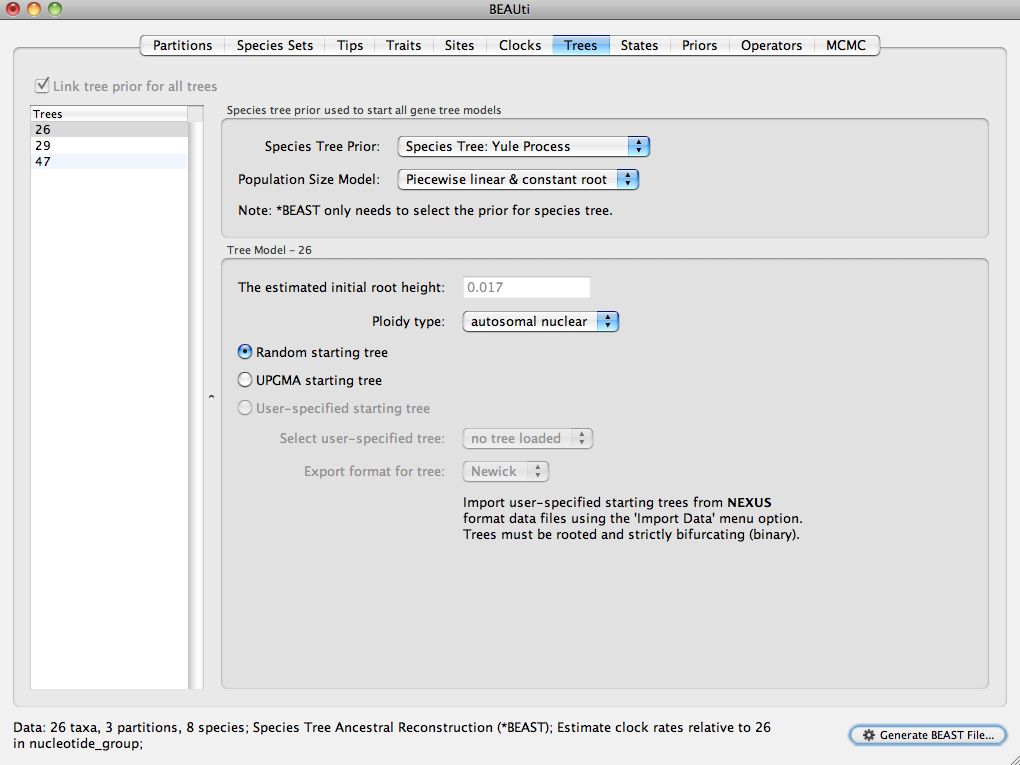
\includegraphics[scale=0.4]{figures/BEAUti_Tree}

\medskip{}

\subsubsection*{Priors and Operators}

The {\bf Priors} panel allows priors to be specified for each parameter in the model. The {\bf Operators} panel is used to configure technical settings that affect the efficiency of the MCMC program (see Notes for details). We leave these two panels unchanged in this analysis.

\subsubsection*{Setting the MCMC options }

The next tab, {\bf MCMC}, provides more general
settings to control the length of the MCMC and the file names. 

Firstly we have the \textbf{Length of chain}. This is the number of
steps the MCMC will make in the chain before finishing. The appropriate length of the chain depends on the size of the data set, the complexity of the
model and the accuracy of the answer required. The default value of 10,000,000
is entirely arbitrary and should be adjusted according to the size
of your data set. For this data set let's initially set the chain
length to 5,000,000 as this will run reasonably quickly on most modern
computers (less than 20 minutes).

The next options specify how often the parameter values in the Markov
chain should be displayed on the screen and recorded in the log file.
The screen output is simply for monitoring the programs progress so
can be set to any value (although if set too small, the sheer quantity
of information being displayed on the screen will actually slow the
program down). For the log file, the value should be set relative
to the total length of the chain. Sampling too often will result in
very large files with little extra benefit in terms of the precision
of the analysis. Sample too infrequently and the log file will not
contain much information about the distributions of the parameters. 
You probably want to aim to store no more than 10,000 samples so this should be
set to no less than chain length / 10,000.

For this exercise we will set the screen log to 10000 and the file log to 1000. The final two
options give the file names of the log files for the sampled parameters and
the trees. These will be set to a default based on the name of the
imported NEXUS file. 

If you would like to save the operator analysis into a file, you need to check  \textbf{Create operator analysis file} which will generate a file with the suffix \texttt{.ops}. 

\medskip{}

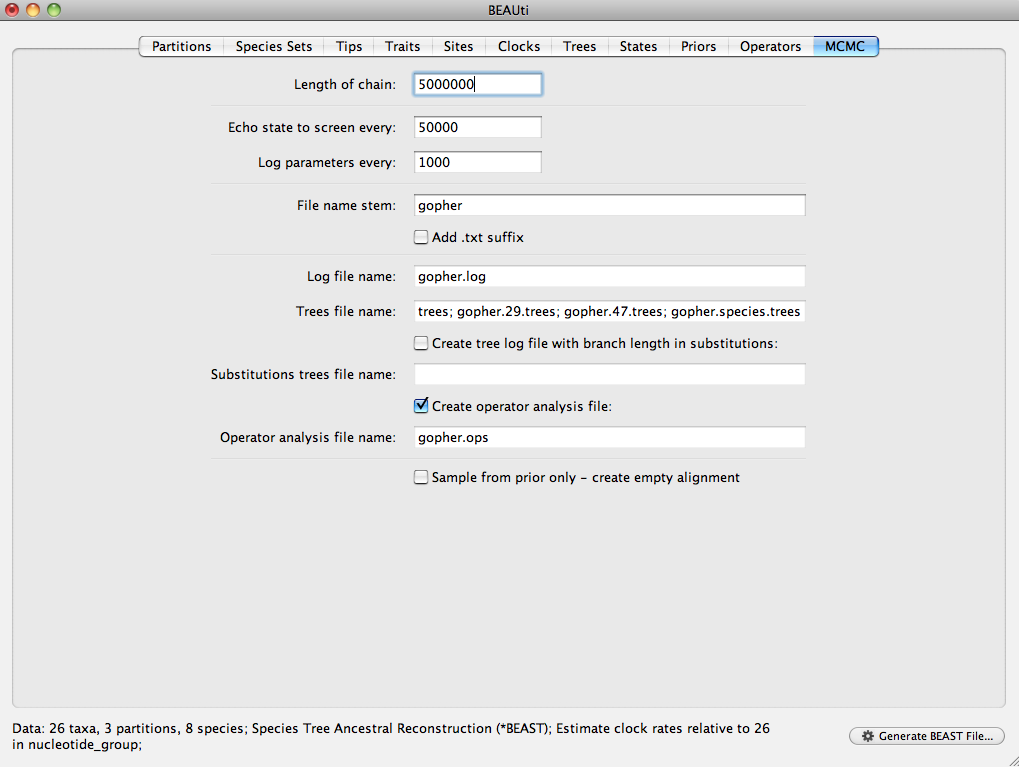
\includegraphics[scale=0.4]{figures/BEAUti_MCMC}

\medskip{}

\begin{itemize}
\item If you are using windows then we suggest you add the suffix \texttt{.txt} to both of these (so,
\texttt{gopher.log.txt} and \texttt{gopher.trees.txt}) so that Windows recognizes
these as text files. 
\end{itemize}

\subsubsection*{Generating the BEAST XML file }

We are now ready to create the BEAST XML file. To do this,
either select the {\bf Generate BEAST File...} option from the \textbf{File} menu or click the similarly labelled button at the bottom of the window. Check the default priors setting and click \textbf{Continue}. Save the file with an appropriate name
(we usually end the filename with \texttt{.xml}, i.e., \texttt{gopher.xml}).
We are now ready to run the file through BEAST. 

\subsection*{Running BEAST }

Now run BEAST and when it asks for an input file, provide your newly
created XML file as input by click \textbf{Choose File ...}, and then click \textbf{Run}. 

\medskip{}

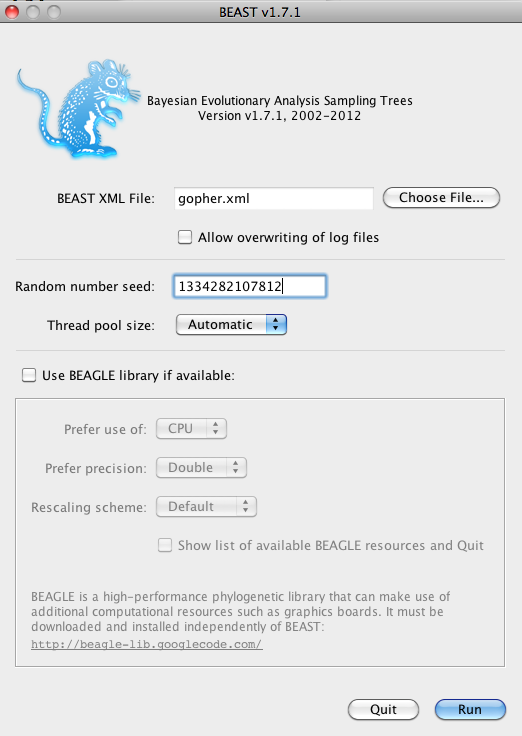
\includegraphics[scale=0.5]{figures/BEAST}

\medskip{}

BEAST will then run until it has finished
reporting information to the screen. The actual results files are
saved to the disk in the same location as your input file. The output to the screen will
look something like this: 

{\scriptsize   
\begin{verbatim}



                   BEAST v1.7.1, 2002-2012
       Bayesian Evolutionary Analysis Sampling Trees
                 Designed and developed by
   Alexei J. Drummond, Andrew Rambaut and Marc A. Suchard
                              
               Department of Computer Science
                   University of Auckland
                  alexei@cs.auckland.ac.nz
                              
             Institute of Evolutionary Biology
                  University of Edinburgh
                     a.rambaut@ed.ac.uk
                              
              David Geffen School of Medicine
           University of California, Los Angeles
                     msuchard@ucla.edu
                              
                Downloads, Help & Resources:
                 	http://beast.bio.ed.ac.uk
                              
Source code distributed under the GNU Lesser General Public License:
            	http://code.google.com/p/beast-mcmc
                              
                     BEAST developers:
	Alex Alekseyenko, Trevor Bedford, Erik Bloomquist, Joseph Heled, 
	Sebastian Hoehna, Denise Kuehnert, Philippe Lemey, Wai Lok Sibon Li, 
	Gerton Lunter, Sidney Markowitz, Vladimir Minin, Michael Defoin Platel, 
          	Oliver Pybus, Chieh-Hsi Wu, Walter Xie
                              
                         Thanks to:
    	Roald Forsberg, Beth Shapiro and Korbinian Strimmer


Random number seed: 1334282107812


Parsing XML file: gopher.xml
  File encoding: MacRoman
Read alignment: alignment1
  Sequences = 26
      Sites = 614
   Datatype = nucleotide
Read alignment: alignment2
  Sequences = 26
      Sites = 601
   Datatype = nucleotide
Read alignment: alignment3
  Sequences = 26
      Sites = 819
   Datatype = nucleotide
Site patterns '26.patterns' created from positions 1-614 of alignment 'alignment1'
  pattern count = 144
Site patterns '29.patterns' created from positions 1-601 of alignment 'alignment2'
  pattern count = 71
Site patterns '47.patterns' created from positions 1-819 of alignment 'alignment3'
  pattern count = 153
Creating the tree model, '26.treeModel'
  initial tree topology = ((((((((((Thomomys_bottae_bottae,Thomomys_monticola_b),Orthogeomys_heterodus),(Thomomys_talpoides_yakimensis,Thomomys_umbrinus_chihuahuae)),Thomomys_bottae_saxatilis),(Thomomys_idahoensis_pygmaeus_a,Thomomys_talpoides_ocius)),Thomomys_townsendii_relictus),(((Thomomys_mazama_nasicus,Thomomys_umbrinus_atroavarius),Thomomys_bottae_laticeps),Thomomys_monticola_a)),((((Thomomys_bottae_alpinus,Thomomys_townsendii_townsendii),Thomomys_bottae_ruidosae),Thomomys_bottae_mewa),(Thomomys_bottae_cactophilus,Thomomys_talpoides_bridgeri))),(Thomomys_bottae_xerophilus,Thomomys_mazama_mazama)),((((Thomomys_bottae_awahnee_a,Thomomys_bottae_awahnee_b),Thomomys_idahoensis_pygmaeus_b),Thomomys_bottae_albatus),Thomomys_bottae_riparius))
  tree height = 0.017
Creating the tree model, '29.treeModel'
  initial tree topology = (((((((((Thomomys_bottae_albatus,Thomomys_bottae_xerophilus),Thomomys_bottae_saxatilis),Thomomys_monticola_a),((Thomomys_talpoides_ocius,Thomomys_talpoides_yakimensis),Thomomys_townsendii_townsendii)),(Thomomys_bottae_awahnee_a,Thomomys_bottae_cactophilus)),Thomomys_umbrinus_chihuahuae),Thomomys_mazama_mazama),((((((Orthogeomys_heterodus,Thomomys_bottae_riparius),(Thomomys_bottae_ruidosae,Thomomys_umbrinus_atroavarius)),Thomomys_talpoides_bridgeri),Thomomys_monticola_b),Thomomys_bottae_laticeps),((Thomomys_bottae_alpinus,Thomomys_mazama_nasicus),Thomomys_bottae_bottae))),(((Thomomys_idahoensis_pygmaeus_b,Thomomys_townsendii_relictus),Thomomys_bottae_awahnee_b),(Thomomys_bottae_mewa,Thomomys_idahoensis_pygmaeus_a)))
  tree height = 0.016
Creating the tree model, '47.treeModel'
  initial tree topology = (((((((((Thomomys_bottae_cactophilus,Thomomys_bottae_saxatilis),(Thomomys_bottae_mewa,Thomomys_townsendii_relictus)),((Thomomys_monticola_b,Thomomys_talpoides_ocius),Thomomys_umbrinus_atroavarius)),Thomomys_bottae_laticeps),(Thomomys_bottae_awahnee_a,Thomomys_townsendii_townsendii)),((Thomomys_bottae_xerophilus,Thomomys_idahoensis_pygmaeus_b),Thomomys_umbrinus_chihuahuae)),(((Orthogeomys_heterodus,Thomomys_mazama_nasicus),Thomomys_bottae_awahnee_b),(Thomomys_bottae_albatus,Thomomys_idahoensis_pygmaeus_a))),Thomomys_bottae_bottae),((((Thomomys_bottae_ruidosae,Thomomys_monticola_a),Thomomys_talpoides_yakimensis),Thomomys_bottae_alpinus),((Thomomys_mazama_mazama,Thomomys_talpoides_bridgeri),Thomomys_bottae_riparius)))
  tree height = 0.017
Using strict molecular clock model.
Using strict molecular clock model.
Using strict molecular clock model.
Creating state frequencies model '26.frequencies': Using empirical frequencies from data = {0.40772, 0.20916, 0.19046, 0.19266}
Creating HKY substitution model. Initial kappa = 2.0
Creating site model.
Creating state frequencies model '29.frequencies': Using empirical frequencies from data = {0.24545, 0.21384, 0.23701, 0.3037}
Creating HKY substitution model. Initial kappa = 2.0
Creating site model.
Creating state frequencies model '47.frequencies': Using empirical frequencies from data = {0.2017, 0.21368, 0.21208, 0.37254}
Creating HKY substitution model. Initial kappa = 2.0
Creating site model.
Loading native NucleotideLikelihoodCore successfully 
TreeLikelihood(26.treeModel) using native nucleotide likelihood core
  Ignoring ambiguities in tree likelihood.
  With 144 unique site patterns.
Branch rate model used: strictClockBranchRates
TreeLikelihood(29.treeModel) using native nucleotide likelihood core
  Ignoring ambiguities in tree likelihood.
  With 71 unique site patterns.
Branch rate model used: strictClockBranchRates
TreeLikelihood(47.treeModel) using native nucleotide likelihood core
  Ignoring ambiguities in tree likelihood.
  With 153 unique site patterns.
Branch rate model used: strictClockBranchRates
Using Yule prior on tree
Likelihood is using -1 threads.
Creating the MCMC chain:
  chainLength=5000000
  autoOptimize=true
  autoOptimize delayed for 50000 steps
# BEAST v1.7.1, r4860
# Generated Fri Apr 13 16:02:42 NZST 2012 [seed=1334282107812]
state	Posterior   	Prior       	Likelihood  	PopMean     	26.rootHeight	29.rootHeight	47.rootHeight	26.clock.rate	29.clock.rate	47.clock.rate
0	-8271.7599  	-408.9912   	-7862.7688  	1.0000      	1.7E-2      	1.6E-2      	1.7E-2      	1.00000     	1.00000     	1.00000     	-
50000	-4402.6081  	-110.7170   	-4291.8911  	0.0093      	2.85227E-2  	2.66503E-2  	1.70572E-2  	1.00000     	0.83166     	1.48458     	0.05 hours/million states
100000	-4282.8572  	5.5473      	-4288.4044  	0.0009      	2.49661E-2  	3.13122E-2  	1.68536E-2  	1.00000     	0.80206     	1.66186     	0.04 hours/million states
150000	-4321.6989  	-32.7608    	-4288.9382  	0.0025      	3.17837E-2  	2.81154E-2  	1.88322E-2  	1.00000     	0.83429     	1.39937     	0.03 hours/million states
200000	-4301.2881  	-12.5667    	-4288.7214  	0.0013      	2.32344E-2  	4.17748E-2  	1.82301E-2  	1.00000     	0.65006     	1.57575     	0.03 hours/million states
250000	-4312.7097  	-9.6236     	-4303.0861  	0.0020      	3.12738E-2  	2.28171E-2  	1.84486E-2  	1.00000     	0.82719     	1.37213     	0.03 hours/million states
300000	-4278.9322  	35.3165     	-4314.2487  	0.0008      	2.27743E-2  	2.26837E-2  	1.82648E-2  	1.00000     	1.19420     	1.46538     	0.03 hours/million states

... ...

4900000	-4276.9360  	17.6994     	-4294.6354  	0.0018      	2.23113E-2  	1.66667E-2  	1.36587E-2  	1.00000     	0.91509     	1.68670     	0.02 hours/million states
4950000	-4238.0976  	49.0728     	-4287.1704  	0.0008      	2.45626E-2  	1.28858E-2  	1.29766E-2  	1.00000     	1.24784     	2.22299     	0.02 hours/million states
5000000	-4304.9506  	-17.2098    	-4287.7408  	0.0017      	2.47898E-2  	3.78072E-2  	2.25424E-2  	1.00000     	0.74967     	1.24236     	0.02 hours/million states

Operator analysis
Operator                                          Tuning   Count      Time     Time/Op  Pr(accept) 
scale(26.kappa)                                   0.36    1106       122      0.11     0.3698      
scale(29.kappa)                                   0.383   1097       91       0.08     0.381       
scale(47.kappa)                                   0.438   1143       131      0.11     0.3596      
scale(29.clock.rate)                              0.485   33005      2668     0.08     0.2684      
scale(47.clock.rate)                              0.568   33415      3546     0.11     0.2804      
up:29.clock.rate 47.clock.rate species.yule.birthRate down:speciesTree species.popMean speciesTree.splitPopSize nodeHeights(26.treeModel) nodeHeights(29.treeModel) nodeHeights(47.treeModel) 0.476   332580     59573    0.18     0.236       
subtreeSlide(26.treeModel)                        0.003   165916     7583     0.05     0.2326      
Narrow Exchange(26.treeModel)                             165585     6047     0.04     0.2971      
Wide Exchange(26.treeModel)                               33216      988      0.03     0.0263      
wilsonBalding(26.treeModel)                               33151      1648     0.05     0.0379      
scale(26.treeModel.rootHeight)                    0.511   33209      1527     0.05     0.2864      
uniform(nodeHeights(26.treeModel))                        331028     17469    0.05     0.5605      
subtreeSlide(29.treeModel)                        0.003   166248     7404     0.04     0.2201      
Narrow Exchange(29.treeModel)                             165728     5610     0.03     0.3173      
Wide Exchange(29.treeModel)                               33262      887      0.03     0.0428      
wilsonBalding(29.treeModel)                               33206      1468     0.04     0.0473      
scale(29.treeModel.rootHeight)                    0.447   33466      1530     0.05     0.2679      
uniform(nodeHeights(29.treeModel))                        330344     16735    0.05     0.5782      
subtreeSlide(47.treeModel)                        0.002   165265     7854     0.05     0.2449      
Narrow Exchange(47.treeModel)                             165918     6217     0.04     0.2445      
Wide Exchange(47.treeModel)                               33011      998      0.03     0.0141      
wilsonBalding(47.treeModel)                               33105      1795     0.05     0.0186      
scale(47.treeModel.rootHeight)                    0.61    33012      1317     0.04     0.2409      
uniform(nodeHeights(47.treeModel))                        332093     17991    0.05     0.5415      
up:down:nodeHeights(26.treeModel)                 0.782   32762      3383     0.1      0.1912      
up:29.clock.rate down:nodeHeights(29.treeModel)   0.766   33152      2502     0.08     0.1841      
up:47.clock.rate down:nodeHeights(47.treeModel)   0.713   32871      3484     0.11     0.1732      
scale(species.popMean)                            0.495   54949      1784     0.03     0.2719      
scale(species.yule.birthRate)                     0.24    33178      1132     0.03     0.3156      
scale(speciesTree.splitPopSize)                   0.171   1037737    40459    0.04     0.2572      
nodeReHeight(sptree,species)                              1036242    39954    0.04     0.295       

6.349283333333333 minutes 

\end{verbatim}}

\subsection*{Analyzing the results}

Run the program called {\bf Tracer} to analyze the output of BEAST. When the main
window has opened, choose {\bf Import Trace File...} from the {\bf File} menu and select the file that
BEAST has created called \texttt{gopher.log}.
You should now see a window like the following:

\medskip{}

\frame{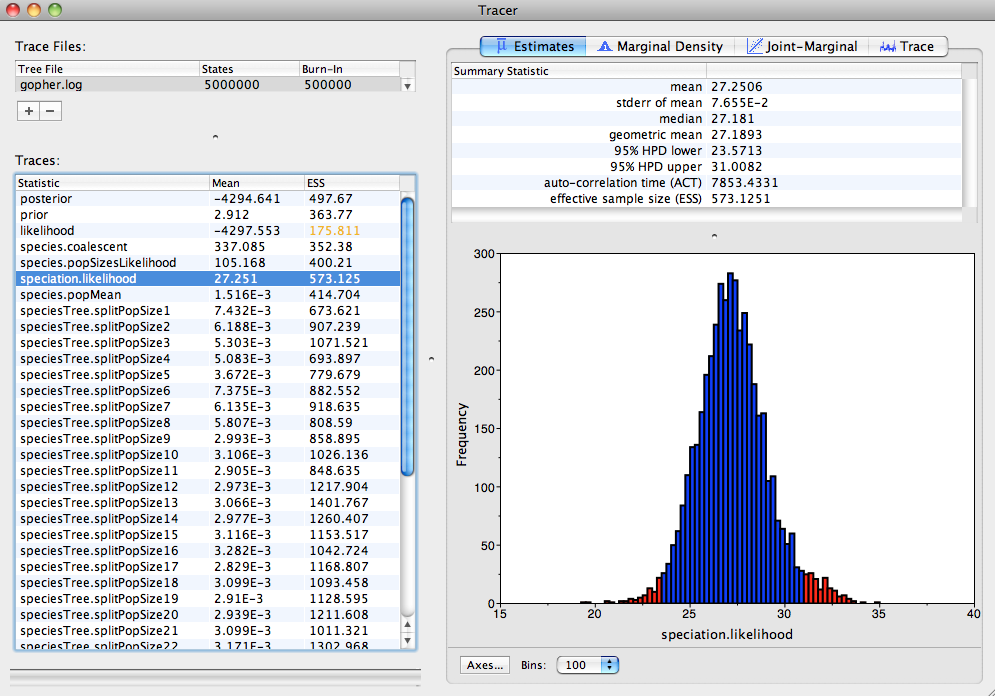
\includegraphics[scale=0.4]{figures/Tracer1}}

\medskip{}

Remember that MCMC is a stochastic algorithm so the actual numbers will not be exactly the same.

On the left hand side is a list of the different quantities that BEAST has logged. There are traces for the posterior (this
is the log of the product of the tree likelihood and the prior probabilities), and the continuous parameters. Selecting a trace
on the left brings up analyses for this trace on the right hand side depending on tab that is selected. When first opened, the
`posterior' trace is selected and various statistics of this trace are shown under the Estimates tab.
In the top right of the window is a table of calculated statistics for the selected trace. 

Tracer will plot a (marginal posterior) distribution for the selected parameter and also give you statistics such as the mean and median. The \texttt{95\% HPD lower} or \texttt {upper} stands for {\it highest posterior density interval} and represents the most compact interval on the selected parameter that contains 95\% of the posterior probability. It can be thought of as a Bayesian analog to a confidence interval. 

Select the \texttt{treeModel.rootHeight} parameter and the next three (hold shift whilst selecting). This will show a display of the
age of the root and the three gene trees. If you switch the tab at the top of the window to {\bf Marginal Density} then you will get a plot of the marginal posterior densities of each of these date estimates overlayed:

\medskip{}

\frame{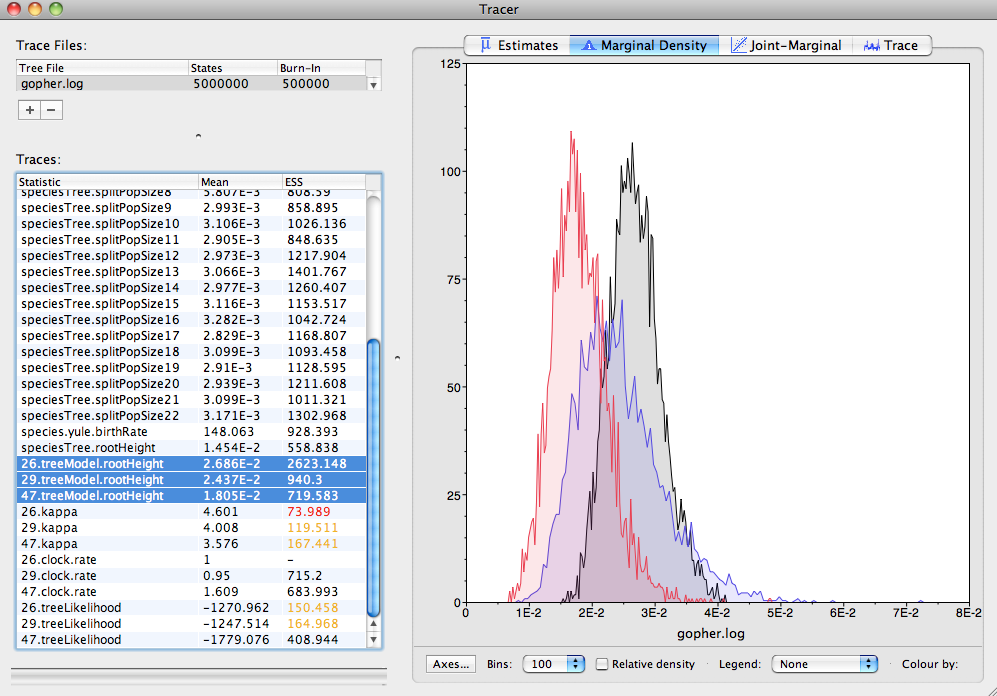
\includegraphics[scale=0.4]{figures/Tracer2}}

\medskip{}

\subsection*{Obtaining an estimate of the phylogenetic tree}

BEAST also produces a sample of plausible trees. 
These need to be summarized using the program {\bf TreeAnnotator} (see Notes for details). This will take the set of trees and identify a single tree that best represents the posterior distribution. It will then annotate this selected tree topology with the mean ages of all the
nodes as well as the 95\% HPD interval of divergence times for each clade in the selected tree. It will also calculate the posterior clade probability for each
node. Run the {\bf TreeAnnotator} program and set it up to look like this:

\medskip{}

\frame{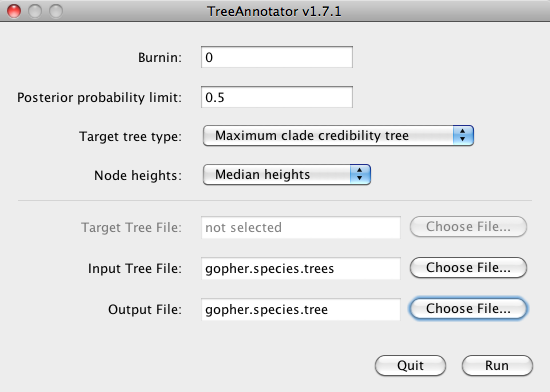
\includegraphics[scale=0.4]{figures/TreeAnnotator}}

\medskip{}

The burnin is the number of trees to remove from the start of the sample. Unlike {\bf Tracer} which specifies the number of
steps as a burnin, in {\bf TreeAnnotator} you need to specify the actual number of trees. For this run, we use the default setting.

The {\bf Posterior probability limit} option specifies a limit such that if a node is found at less than this frequency in the sample
of trees (i.e., has a posterior probability less than this limit), it will not be annotated. The default of 0.5 means that only nodes
seen in the majority of trees will be annotated. Set this to zero to annotate all nodes.

For {\bf Target tree type} you can either choose a specific tree from a file or ask TreeAnnotator to find a tree in your sample.
The default option, {\bf Maximum clade credibility tree}, finds the tree with the highest product of the posterior probability of
all its nodes.

Choose {\bf Mean heights} for node heights. This sets the heights (ages) of each node in the tree to the mean height across the
entire sample of trees for that clade.

For the input file, select the trees file that BEAST created (by default this will be called \texttt{gopher.species.trees}) and select a file for the
output (here we called it \texttt{gopher.species.tree}).

Now press \texttt{Run} and wait for the program to finish.

\subsection*{Viewing the Tree}
Finally, we can look at the tree in another program called {\bf FigTree}. Run this program, and open
the \texttt{gopher.species.tree} file by using the Open command in the File menu. The tree should appear.
You can now try selecting some of the options in the control panel on the left. Try selecting
{\bf Node Bars} to get node age error bars. Also turn on {\bf Branch Labels} and select {\bf posterior} to get
it to display the posterior probability for each node. Under {\bf Appearance} you can also tell FigTree
to colour the branches by the length.
You should end up with something like this:

\medskip{}

\frame{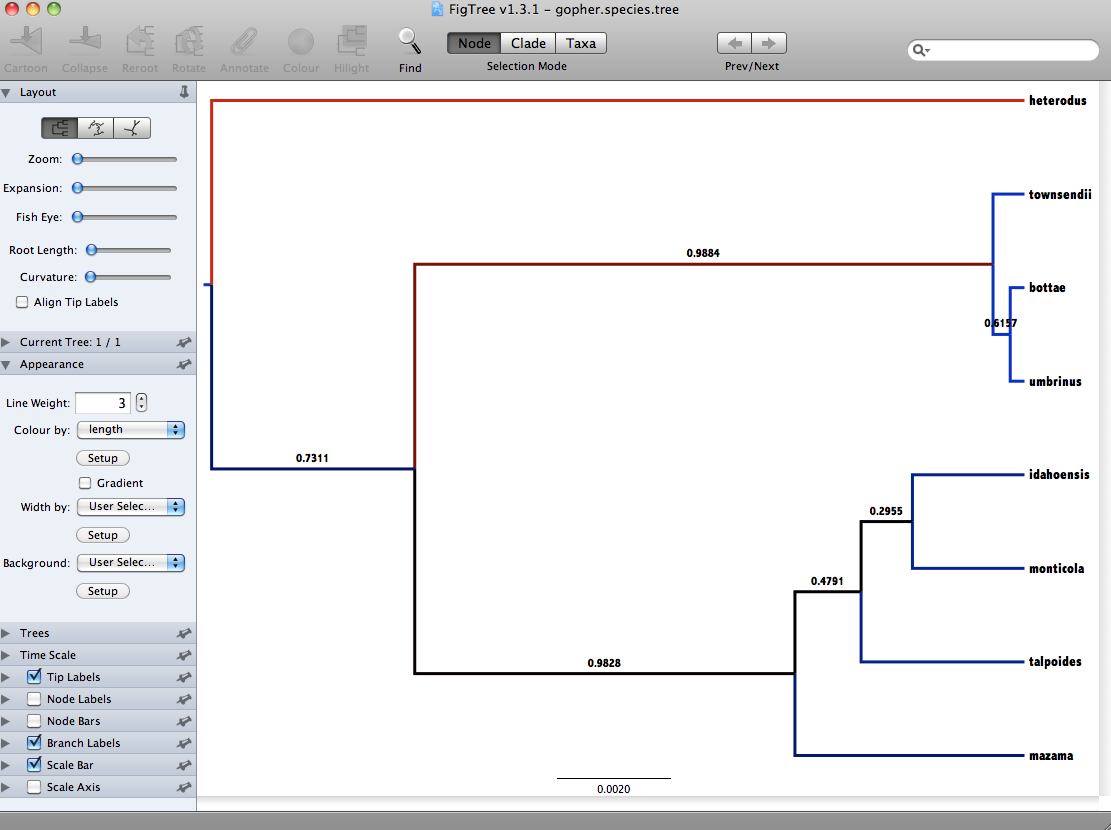
\includegraphics[scale=0.4]{figures/FigTree}}

\medskip{}

\subsection*{Comparing your results to the prior}

Using BEAUti, set up the same analysis but under the MCMC options, select the {\bf Sample from prior only} option. This will allow you to visualize the full prior distribution in the absence of your sequence data. Summarize the trees from the full prior
distribution and compare the summary to the posterior summary tree.

%\bibliographystyle{plainnat} 
%\bibliographystyle{ieeetr} 
%\bibliographystyle{named}
%\bibliographystyle{acm} 
\bibliographystyle{amsplain} 
%\bibliographystyle{agsm}
\bibliography{STARBEAST}

\end{document}
